\section{Algorithmen}
\label{sec:algorithmen}

Zur Auswertung der gesammelten Messaden werden wie in Abbildung
\ref{fig:algo} gezeigt, bestimmte Algorithmen benötigt, um die
Position zu bestimmen. Zwei Grundlegende Methoden zur Bestimmung der
Position sind \textbf{Triangulation} und \textbf{Trilateration}, die
die Grundlage zu anderen Verfahren bilden.


\subsection{Triangulation}

Wird das \ac{AoA} Verfahren verwendet müssen mindestens zwei ortsfeste
Koten $A$ und $B$ so wie die Einfalswinkel $\alpha$ und $\beta$ der
Signale bekannt sein. Dann kann mittels Triangulation (Abbildung
\ref{fig:triang}) die Position eines weiteren Knoten $C$ berechnet
werden. Der Knoten $C$ kann wiederum ein stationärer oder ein mobieler
Knoten sein.

\begin{figure}[h!]
  \centering
  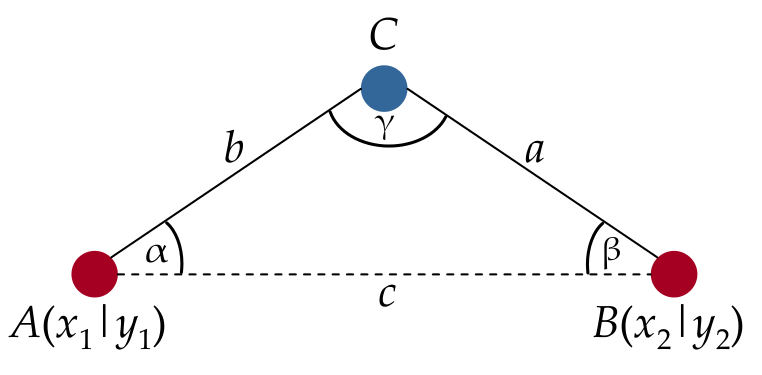
\includegraphics[scale=0.3]{img/triang}

  \caption{Triangulation}
  \label{fig:triang}
\end{figure}

Der Grundgedanke dabei ist, dass theoretisch mit nur zwei bekannten,
ortsfesten Knoten, die Position aller Nachbarn berechnet werden kann.
Sind dabei alle Knoten stationär, ist dies auch möglich, bei mobielen
Knoten kann dies allerdings Problematisch werden, da die Position des
Knotens sich permanent verändern kann. Zudem ist die Genauigkeit der
Triangulation bei mobilen Sensoren sehr schlecht und die Position kann
durch den hohen Messfehler nicht exakt bestimmt werden.
\cite{roehrig2009} 

Die Berechnung mittels Triangulation ist für einen \ac{uC} nicht sehr
aufwendig, da sie nur den Sinus- oder Cosinussatz verwendet. (Gleichung
\ref{eq:triang})

\pagebreak
\begin{framed}
\begin{equation}
  \label{eq:triang}
  c = \sqrt{(B_{x)} - A_{x})^2 + (B_{y} - A_{y})^2}
  ~~~~~~~~
  \varphi = arctan(\frac{B_{y} - A_{y}}{B_{x}} - A_{x})
\end{equation}
\begin{equation*}
  b = c \cdot \frac{sin(\beta)}{sin(\alpha + \beta)}
\end{equation*}
~\\
\begin{equation*}
  C_{x} = A_{x} + b \cdot cos(\varphi)
  ~~~~~~~~
  C_{y} = A_{x} + b \cdot sin(\varphi)
\end{equation*}
\end{framed}
\myequations{Triangulation}


\subsection{Trilateration}

Werden Verfahren wie \ac{ToA}, \ac{TDoA} oder \ac{RToF} eingesetzt,
sind die Winkel der Signale nicht bekannt. Hier werden mindestens
drei ortsfeste Knoten benötigt, um die Position zu einem weiteren
Knoten zu berechnen. Ein weiterer Vorteil der Trilateration ist, dass
die Hardware Anforderungen zur Messung des Einfallwinkels wesentlich
höher sind, als eine reine Distanzmessung. \cite{roehrig2009} 

\begin{figure}[h!]
  \centering
  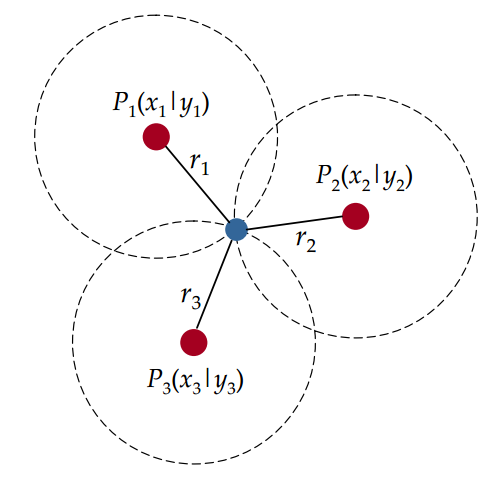
\includegraphics[scale=0.5]{img/trilat}

  \caption{Trilateration}
  \label{fig:trilat}
\end{figure}

Für die Distanz zu den Knoten $P_{¹}$, $P_{2}$ und $P_{3}$ gilt:

\begin{framed}
\begin{equation}
  \label{eq:trilat1}
  r_{i} = \sqrt{(p_{x} - x_{i})^{²} + (p_{y} - y_{i})^{2}}
\end{equation}
\end{framed}
\myequations{Trilateration: Distanz zu stationären Knoten}

Die Position des vierten Knoten lässt sich dann über das
Gleichungssystem \ref{eq:trilat2} berechnen.

\begin{framed}
\begin{equation}
  \label{eq:trilat2}
  \begin{pmatrix}
    P_{x} \\
    P_{y}
  \end{pmatrix}
  =
  H^{-1} \cdot z
\end{equation}
\begin{equation*}
  H = 
  \begin{bmatrix}
    2 \cdot x_{1} - 2 \cdot x_{2} & 2 \cdot y_{1} - 2 \cdot y_{2} \\
    2 \cdot x_{1} - 2 \cdot x_{3} & 2 \cdot y_{1} - 2 \cdot y_{3}
  \end{bmatrix}
\end{equation*}
\begin{equation*}
  z = 
  \begin{pmatrix}
    r_{2}^2 - r_{1}^2 + x_{1}^2 - x_{2}^2 + y_{1}^2 - y_{2}^2 \\
    r_{3}^2 - r_{1}^2 + x_{1}^2 - x_{3}^2 + y_{1}^2 - y_{3}^2
  \end{pmatrix}
\end{equation*}
\end{framed}
\myequations{Trilateration: Gleichungssystem}


\subsection{Weiterführende Algorithmen}

Wie bereits beschrieben, bieten die beiden geziegten Verfahren nur
ungenaue Ergebnisse, vor allem bei mobielen Knoten ist der Fehler sehr
groß. Auß diesem Grund werden weitere Verfahren benötigt, um die
Wahrscheinlichkeit zu maximieren, dass die berechnete Position stimmt.


\subsubsection{Klassische Schätzer: Maximum likelihood}

Unter der Annahme, dass alle Messfehler unabhängig und Gleichverteilt
sind und die \ac{PDF} $p_{M_{ij}}(m_{ij} \vert X)$ mit $X
= \begin{bmatrix}X_{1}, ..., X_{m}\end{bmatrix}^{\top} \in
\mathbb{R}^{2 \times M}$ ist, kann die Schätzfunktion wie folgt
geschrieben werden.

\begin{framed}
  \begin{equation}
    \label{eq:maxlike}
    \hat H = \arg \max_{X \in \mathbb{R}^{2 \times M}} \sum_{i=1}^{M}
    \sum_{j \in \alpha_{i} \bigcup \beta_{i}} \log p_{M_{ij}}(m_{ij}
    \vert X)
  \end{equation}
\end{framed}
\myequations{Maximum likelihood}

Der Schätzer ist asymptotisch effizient, dafür wird aber eine
komplette Statistik der Messfehler benötigt. Aus diesem Grund ist es
in der Praxis meist nicht möglich, alle \textit{a priori}
Wahrscheinlichkeiten \ac{uC} zu halte.

Da das \ac{ML} Problem NP-Vollständig ist, kann man keine Aussage
darüber treffen, ob es in einer \textit{guten} Zeit eine brauchbare
Lösung findet. Darum gibt es weitere Ansätze, so kann das \ac{ML}
Problem z.B. in ein \ac{SDP}s Problem umgewandelt werden. Desweiteren
gibt es Ansätze, das Problem in Probleme der Mengenlehre umzuformen.
Dabei ergibt sich dann z.B. ein \ac{CFP}. Auf dem meisten kleinen
Knoten, sind dann diese Berechnungen allerdings nicht mehr einfach
durchführbar. \cite{gholami2011}


\subsubsection{Erweiterter Kalman Filter}

Die bereits beschriebene \textit{Trilateration} kann auch durch einen
\ac{EKF} verbessert werden. Dieser berechnet rekursiv die Position des
Punktes anhand der Messadaten und verwendet dabei einen Prädikt-ions
und einen Korrektur-Schritt um die Schätzung zu verbessern und den
Messfehler auszugleiuchen. Diese Methode ist vorallem bei mobielen
Knoten sehr hilfreich wie in der Abbildung \ref{fig:ekf} zu erkennen
ist.

\begin{figure}[h!]
  \centering
  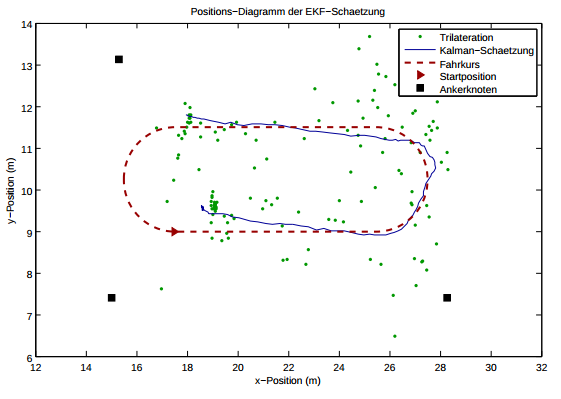
\includegraphics[scale=0.7]{img/kalman}

  \caption{Erweiterter Kalman Filter}
  \label{fig:ekf}
\end{figure}

\newpage
Der \ac{EKF} arbeitet dabei mit folgenden drei Schritten:

\begin{enumerate}
\item \textbf{Prädiktion} -- Es wird eine Vorhersage der Position des
  Knotens bestimmt.
\item \textbf{Messung} -- Die Position wird mittels der
  Trilateration gemessen.
\item \textbf{Korrektur} -- Die Daten der \textit{Prädiktion} und
  \textit{Messung} werden miteinander Abgeglichen.
\end{enumerate}

\begin{figure}[h!]
  \centering
  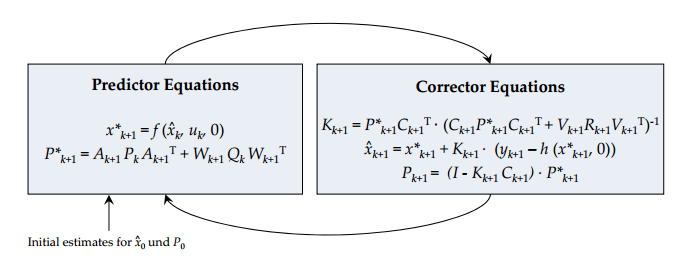
\includegraphics[scale=0.6]{img/kalman2}

  \caption{Schritte des - Erweiterter Kalman Filter}
  \label{fig:ekf}
\end{figure}

Der Vorteil des \ac{EKF} ist hier, dass die Positionsbestimmung zu
Beginn zwar noch sehr Ungenau ist, da noch kaum Messadaten vorhanden
sind, diese duch den Korrekturschritt aber immer besser wird.

Ein System, bei dem solche Verfahren zum Einsatz kommen sind z.B. die
\ac{FTS} des Unternehmens \textit{MLR System GmbH}, dabei kann ein
Fahrzeug über ein Sensornetz gesteuert selbständig seine Aufgaben
erledigen. Die Abbildung \ref{fig:fg} zeigt z.B. einen fahrerlosen
Gabelhubwagen der diesen Anforderungen entspricht.

\begin{figure}[h!]
  \centering
  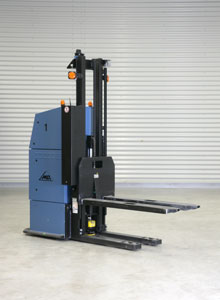
\includegraphics[scale=1.0]{img/Fahr_Gabelhubwagen}

  \caption{Fahrerloser Gabelhubwagen}
  \label{fig:fg}
\end{figure}
